\documentclass{article}
\usepackage[utf8]{inputenc}
\usepackage[T1]{fontenc} 
\usepackage[french]{babel}
\usepackage{graphicx}
\usepackage{subfigure}
\usepackage[table]{xcolor}
\usepackage{geometry}
\usepackage{hyperref}
\usepackage{appendix}
\usepackage{pdfpages}

\geometry{hmargin=2.5cm,vmargin=3cm}
\setlength{\parskip}{0.1cm}

\title{Rapport de Stage}
\author{Laureline MARTIN}
\date{Mercredi 7 Octobre 2020}

\begin{document}
\maketitle
\vspace*{14cm}
\begin{center}
	\textbf{Encadrants :}
\end{center}
\begin{tabular}{p{4cm}p{4cm}p{8cm}}
	\hspace*{-1cm}
	Mme. Viviane GAL & Ingénieure & Equipe \textit{Interactivité pour lire et jouer - ILJ}\smallskip\\
	\hspace*{-1cm}
	M. Eric GRESSIER-SOUDAN & Professeur des universités & Equipe \textit{Réseaux et Objets Connectés - ROC}
	\smallskip\\
	\hspace*{-1cm}
	Mme. Elena KORNYSHOVA & Maître de conférences & Equipe \textit{Igénieurie des systèmes d'information et de décision - ISID}
\end{tabular}


\newpage
\begin{center}
	\textbf{Résumé :}
\end{center}
\hspace*{0.4cm}
Durant cinq mois et demi, j'ai travaillé au laboratoire de recherche CEDRIC au Conservatoire National des Arts et Métiers de Paris.\par
Ce stage s'est inscrit au sein du projet exploratoire "Conception et développement des jeux pervasifs adaptables avec la prise en compte des états émotionnels des joueurs" du laboratoire.
L'objectif global de ce projet est de proposer un jeu pervasif où le joueur et ses émotions sont au coeur même du jeu. 
Pour cela, des capteurs physiologiques sont utilisés pour détecter et reconnaître les états émotionnels du joueurs ainsi que des capteurs placés dans l'environnement pour connaître le contexte global. 
Ces capteurs génèrent beaucoup de données qu'il faut traiter en temps-réel pour une adaptation dynamique du jeu.
Dans ce rapport, nous prposons une solution pouvant ingérer les données provenant de capteurs physiologiques en temps-réel.
Ensuite, cette solution envoie ces données à des algorithmes déjà existant qui permettent de déduire des états émotionnels.
Un état de l'art ainsi qu'une première version d'une ontologie afin de répondre à cet objectif ont été proposées et se trouvent dans ce rapport. 
\bigskip\newline
\begin{center}
	\textbf{Abstract :}
\end{center}
\hspace*{0.4cm}
I worked for the CEDRIC research laboratory based on Conservatoire Nationnal des Arts et Métiers at Paris during five mounths and half.\par
This work was for the laboratory's exploratory project "Desing and development of adaptables pervasives games to players' emotional states".
The main project goal is to develop a pervasive game where player and his emotions are the heart of the game.
To reach this goal, physiological sensors are used in order to detect and recognize player's emotional states and others sensors are placed in environment to know the global context.
Sensors generate a lot of data that must be processed in real-time to a dynamic game's adaptation.
This report contains a solution to ingest real-time physiological sensors' data.
This solution sends data to existing detection and recognition of emotional states algorithms.
This report contains a state of the art and a first version of an ontology that I made too. 
\vspace*{3cm}
\begin{center}
	\textbf{Avant-propos}
\end{center}
\hspace*{0.4cm}
Dans le cadre de la validation du Master 2 Data Managment in a Digital World - Datascale, proposé par l'Université de Versailles Saint-Quentin / Paris Saclay, j'ai effectué un stage de cinq mois et demi du 16 Mars 2020 au 30 Septembre 2020.
Le contexte particulier lié à la crise sanitaire m'a amené à travailler pour la majorité de mon stage en télétravail (du 16 Mars au 10 Septembre).\par
Pour communiquer pendant cette période de travail à distance, nous utilisions les mails et nous avons organisé des réunions via Teams tous les 7 à 15 jours.
Ces réunions duraient entre une demie heure et une heure.
Ces sessions vidéos étaient l'occasion de faire le point sur l'avancement de mon travail et sur les tâches des jours à venir.
Cependant, la barrière de l'écran a créé un réel manque de spontanéité lors de nos échanges.
Pour ma part, je pense que les visio-conférences n'ont pas suffit pour échanger tout au long de cette période de télétravail. 
Peut-être qu'une autre forme de communication, comme une messagerie instantanée, ajoutée à celle des réunions sur Teams, aurait pu réduire se manque de spontanéité.\par
A l'issue de ce stage, je pense que les réunions en présentiel restent la meilleure manière de communiquer et de partager autour d'un projet.

\newpage
\renewcommand{\contentsname}{Table des matières}\tableofcontents

\newpage
\section{Introduction}
	Depuis plusieurs années, les jeux pervasifs se multiplient sur le marché, proposant aux joueurs des conetnus très immersifs.
	Le jeu pervasif (aussi appelé jeu omniprésent) est un genre de jeu qui mêle le monde physique et le monde numérique et rend floue cette frontière.
	% Comme le décrit Astic dans \cite{astic_2013},
	Dans le jeu pervasif, le contexte est essentiel. 
	Quatre facteurs sont mis en jeu : l'espace, le temps, la technologie et les rapports sociaux. 
	L'espace du jeu pervasif est à la fois ancré dans le réel et à la fois virtuel.
	Il convient alors que des ponts existent entre ces deux espaces. 
	Ces ponts peuvnet se faire via des objets, des points géographiques, des personnes, etc. 
	Le temps est calqué sur le temps réel mais il peut être utilisé de différentes manières. 
	L'heure et/ou le jour peuvent influencer le comportement que doit adopter le joueur.
	La technologie est également importante. 
	Elle doit rester accessible au joueur, tant sur le plan pratique que sur le plan financier. 
	La géolocalisation, les réseaux sans fil, etc. sont des technologies utilisées pour ce type de jeu.
	Dans les jeux pervasifs, les joueurs, les spectateurs et les non-joueurs sont mélangés sur le même espace. 
	Les joueurs n'ont pas de caractéristiques particulières pour se reconnaître.%\par
	Le jeu pervasif à un un impact social et culturel important.
	Il favorise les récontres dans l'espace physique.
	Il permet de découvrir de nouveaux endroits, de nouvelles choses et de s'enrichir culturellement.
	Cependant, le jeu omniprésent ne met pas réellement le joueur au centre de jeu.\par
	Le projet "" vise à meettre le joueur et ces émotions au centre du jeu.
	C'est les émotions du joueurs qui influenceront les événements du jeu.
	Pour pouvoir détecter et reconnaître les ététs émotionnels du joueur afin que le jeu s'y adapter et propose l'événement le plus adéquant, de multiples capteurs physiologiques doivent être utilisés.
	Ces capteurs généèrent beaucoup de données qui doivent stockées et traités.
	Ces données permettront à des a des algorithmes de reconnaître les états émotionnels.\par
	Le but de ce travail a été de dresser le contour et d'affiner le conceptualisation d'un jeu pervasif adaptable aux états émotionnels du joueur. 
	Dans ce rapport, nous nous sommes intéressés, d'une part, à l'adaptation de jeu selon le contexte émotionnel et d'autre part, à la gestion de données générées par les capteurs physiologiques.\par
	Nous allons tout d'abord présenter l'état de l'art présentant différentes approches pour l'adaptation dynamique d'un jeu pervasif aux états émotionnels du joueur.
	Nous aborderons l'expérience que nous avons mené lors d'un escape game et la notion d'expérience .
	Puis nous présenterons une ontologie non-aboutie d'un jeu pervasif prenant en compte l'état émotionnel du joueur.
	Enfin nous présenterons une solution pour la gestion de données provenant de capteurs physiologiques

\section{Le projet}
	Le projet exploratoire initié par trois enseignants-chercheurs du laboratoire CEDRIC du CNAM de intitulé "Conception et développement des jeux pervasifs adaptables avec la prise en compte des états émotionnels des joueurs" vise à élaborer un jeu pervasif capable de s'adapter dynamiquement selon le contexte du joueur et son environnement.
	\subsection{Motivations et objectifs du projet}
		Le but est de concevoir un jeu omniprésent capable de détecter et de reconnaître dynamiquement l'état émotionnel courant de joueur. 
		Il faut aussi que le jeu puisse s'adapter à cet état en temps-réel en proposant un événement spécifique. 
		Cet événement devra soit 
		\begin{itemize}
			\item avoir tendance à provoquer le même état émotionnel que celui expérimenté par le joueur à cet instant afin de le maintenir dans cet état émotionnel,
			\item avoir tendance à provoquer un autre état émotionnel que celui expérimenté par le joueur à cet instant dans le but de provoquer un changementd'état émotionnel.
		\end{itemize}
		Le choix de maintenir ou de changer l'état émotionnel du joueur devra se faire selon différents critères tels que le type de l'état émotionnel (positif ou négatif), l'avancement dans le jeu ou bien le contexte environnemental courant.\par
		Toutefois, la conception d'un tel jeu devra rester assez générique pour pouvoir l'appliquer à d'autres domaines dans de prochains projets.
	\subsection{La problématique}
		Dans ce rapport, nous allons traiter principalement la problématique de la gestion des données générées par les capteurs physiologiques.
		Pour atteindre notre objectif final, il est important de pouvoir utiliser les données des capteurs pour déterminer les états émotionnels afin que le jeu puisse s'y adapter. Cela pose une contrainte importante sur la gestion des données en temps-réel.
		En effet, la réponse à l'état émotionnel courant du joueur doit être la plus immédiate possible afin de ne pas créer un sentiment de décalage entre le ressenti du joueur et l'adaptation du jeu.
	\subsection{Sujets connexes}
		Pour répondre à cette problématique, nous avons besoin d'avantage de contexte sur des sujets connexes tels que : les méthodes de détections et de reconnaîssance des états émotionnes, la notion d'expérience utilisateur et le jeu pervasif.

\section{Etat de l'art}
	Notre état de l'art s'intéresse aux différentes méthodes déjà existantes dans la littérature scientifique permettant à différents types de jeux de s'adapter aux états émotionnel de leurs joueurs.\par
	Dans l'état de l'art, nous proposons un cadre que nous avons conçu pour comparer des approches pour l'adaptation de jeux aux états émotionnels des joueurs. Le cadre s'appuie sur les critères suivants :
	\begin{itemize}
		\item Les méthodes pour la détection et pour la reconnaissance des états émotionnels
		\begin{itemize}
			\item Les capteurs utilisés
			\item Les algorithmes utlisés pour la détection et/ou la méthode de l'état émotionnel
		\end{itemize}
		\item Les autres caractéristiques de l'utilisateur prises en compte par le jeu
		\item Les méthodes d'adaptation d'un jeu au contexte de son utilisaeur
		\begin{itemize}
			\item Méthodes pour l'adaptation du jeu selon l'état émotionnel du joueur
			\item Méthodes pour l'adaptation du jeu selon d'autres caractéristiques du joueur
		\end{itemize}
	\end{itemize}
	L'état de l'art se trouve en Annexe \ref{ann:eda}.\par
	De cette comparaison, il en ressort plusieurs questions et limites.
	Tout d'abord, on remarque que seulement quelques états émotionnels sont raités dans les approches. 
	Même si on peut imaginer que certains états émotionnels ne seront jamais expérimenté au cours du jeu que nous souhaitons concevoir, il semble tout de même important de pouvoir prendre en compte le plus grand nombre d'états émotionnels possible.
	Sans quoi, nous le jeu pourrais mal s'adapter au joueur et impacter négativement son niveau d'intérêt pour le jeu.
	Dans notre cas, nous utilisons des capteurs physiologiques de contact, c'est-à-dire collé au joueur, pour aquérir des données sur son état physiologique pour déduire son état émotionnel courant via des algorithmes.\par
	On observe que certaines aproches font aussi cela en utilisants différents types d'algorithmes mais que d'autres utilises des modèles pour "prédire" l'état émotionnel courant du joueur.
	Ce genre de méthode peut être intéressante car elle retire l'équipement de capteurs du joueur.
	Cependant, ce type de méthode semble être moins précise car elle se base sur le principe que tous les joueurs ressentirons exactement le même état émotionnel lorsqu'ils se retrouveront dans le même cas de figure.
	De plus, cela implique d'envisage absolument tous les états du jeu possibles, toutes les actions possibles et d'associer un état émotionnel pou chacque intersection.
	Ce qui nous fait croire que l'utilisation de capteurs physiologiques, même si c'est plus contraignant pour le joueur, est plus pertinent.\par
	D'autres critères peuvent être considérés pour augmenter la connaissance sur le joueur.
	Ces caractéristiques peuvent être intéressantes à étudiant à la fois pour la détection et la reconnaissance de l'état émotionnel mais aussi pour l'enrichissement de la connaissance du contexte de l'environnement globale. 
	Ces caractéristiques peuvent aussi bien s'appuyer sur un questionnaire de préférence rempli par l'utilisateur que sur la présence de capteurs dans l'environnement.


\section{Expérience d'un Escapte Game}

\section{Prototypage}

\section{Conclusion}



\newpage
\appendix
\section{Annexe 1 : Offre de stage}\label{app:annexe1}
	\textbf{Elaboration du modèle conceptuel des jeux pervasifs adaptables avec la prise en compte des états émotionnels des joueurs}\par
	\medskip
	\textbf{Contexte :}\newline
	Le champ des jeux affectifs est nouveau. Il s’appuie sur l’intégration de nouveaux moyens à développer dans les jeux afin d’adaptabilité. [1] et [2] présentent une méthodologie unifiée pour la conception des jeux affectifs utilisant le plus tôt possible le mécanisme de boucle émotionnelle. Ils repèrent des variations à l’aide de mesures physiologiques et appliquent un modèle issu d’un ensemble construit considéré comme en relation avec les émotions. Leur étude montre combien la dimension émotionnelle de l’utilisateur est importante mais difficile à gérer.\newline
	Le profil du joueur, y compris ses émotions, impacte la conception des jeux. Afin de proposer une meilleure expérience aux joueurs et de proposer un jeu particularisé, le jeu doit être adaptable en fonction du contexte global du joueur. Nous sommes dans une approche holistique qui combine à la fois l’individu et ses émotions, et, les influences de l’entourage qui va du bâtiment lui-même à l’atmosphère que dégage le lieu. Très peu de travaux ont été faits pour la conception et le développement des jeux adaptables dynamiquement. [3] formalise le concept des jeux appliqués aux visites de musées. Ce travail modélise le jeu de visite et propose un processus d’équilibrage entre la dimension ludique et la dimension non ludique (la visite) de ce type de jeux. [3] propose des patrons de mission qui servent d’éléments réutilisables lors de la conception des jeux, mais qui ne couvrent qu’une partie du processus de conception.\par
	\textbf{Sujet :}\newline
	Il s’agit dans ce stage d’élaborer un modèle conceptuel du jeu pervasif adaptable basé sur les émotions. Ce modèle, éventuellement réalisé sous forme d’une ontologie, doit couvrir toute la variété des facteurs qui impactent le jeu tels que le profil de l’utilisateur et ses données physiologiques exprimant son état émotionnel. Cette ontologie doit être construite de façon à ce qu’elle soit adaptée à la démarche situationnelle nécessaire pour la composition dynamique du jeu.

\section{Annexe 2 - Adaptation d’un jeu pervasif particularisé basée sur l'état émotionnel et sur les caractéristiques du joueur – État de l’art}\label{ann:eda}
	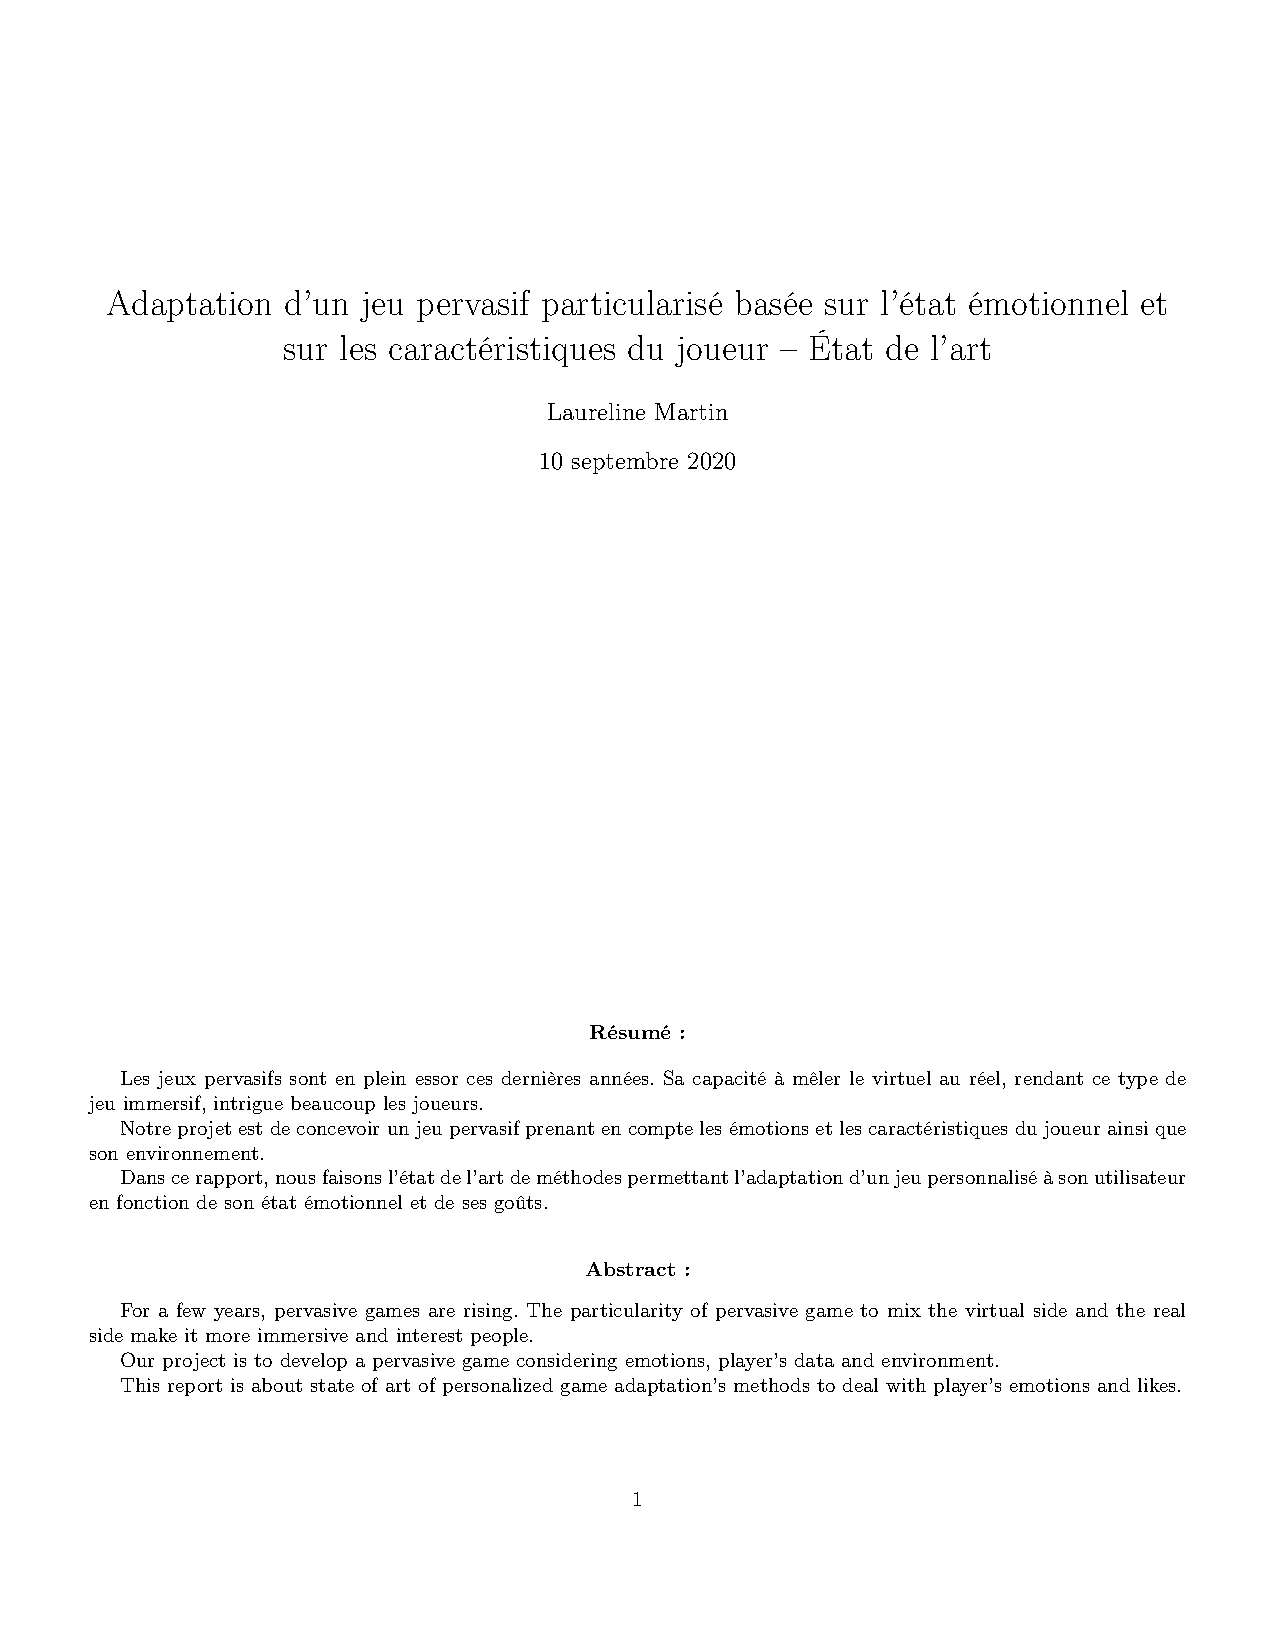
\includepdf[pages=-]{../include/eda.pdf}

%\section{Annexe 3 - Les classes en détail}\label{ann:detailclasse}
%	\includepdf[pages=-]{../include/classes.pdf}

%\section{Annexe 4 - Synthèse comparative entre Kafka et RabbitMQ}%\label{ann:kafkarabbitmq}
%	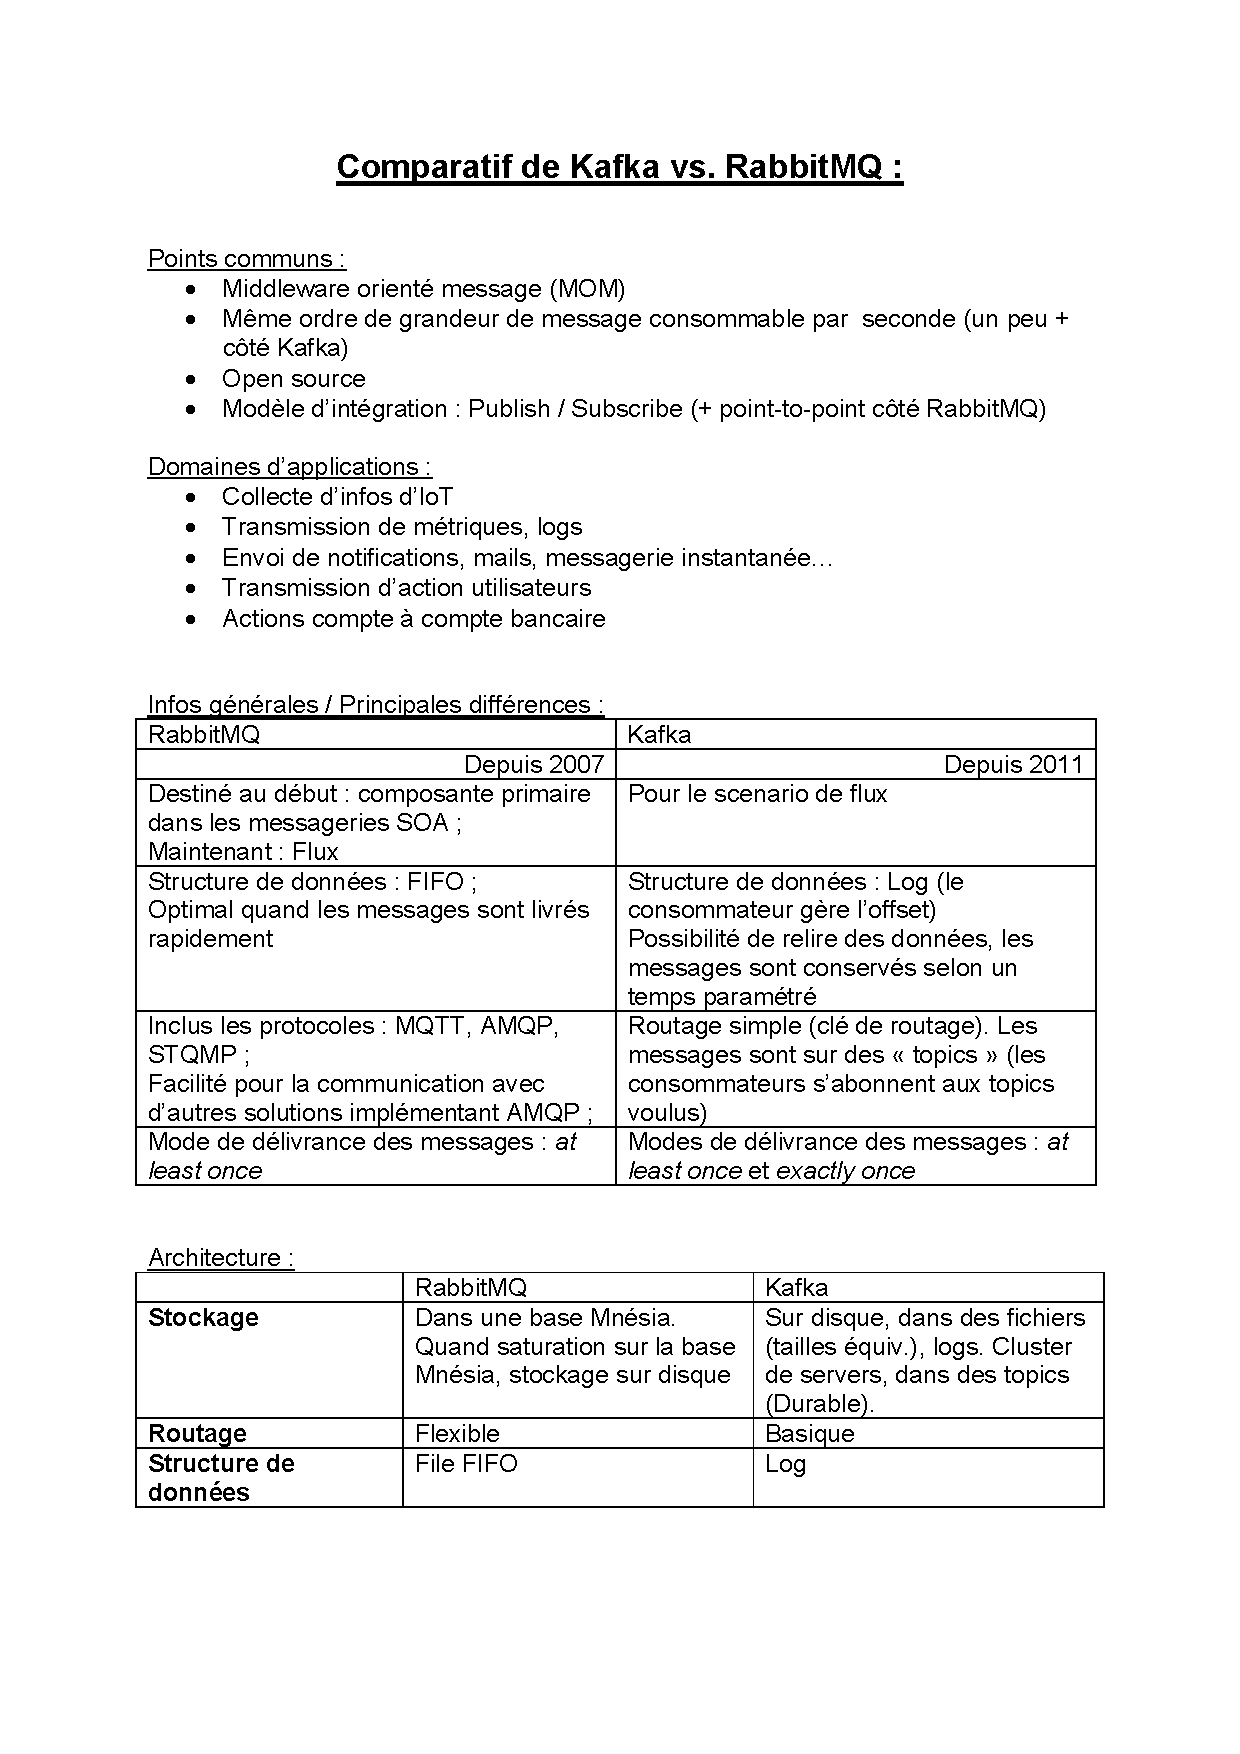
\includepdf[pages=-]{../include/comparatifKafkaVSRabbitMQ.pdf}	

\bibliographystyle{abbrv}
\bibliography{../include/biblio}
\end{document}